\subsection{Python}
\subsubsection{Python là gì}

\begin{center}
  \captionsetup{type=figure}
  \includesvg[width=12cm]{img/python.svg}
  \captionof{figure}{Python}
\end{center}

Python là một ngôn ngữ thông dịch bậc cao, đa mục đích được tạo bởi Guido van Rossum vào năm 1991. Python được thiết kế với ưu điểm mạnh là dễ đọc, dễ học và dễ nhớ. Python là ngôn ngữ có hình thức rất sáng sủa, cấu trúc rõ ràng, thuận tiện cho người mới học lập trình. Cấu trúc của Python còn cho phép người sử dụng viết mã lệnh với số lần gõ phím tối thiểu.
\subsubsection{Đặc điểm của Python}
\begin{itemize}
    \item \textbf{Ngôn ngữ lập trình đơn giản, dễ học:} Python có cú pháp rất đơn giản, rõ ràng. Nó dễ đọc và viết hơn rất nhiều khi so sánh với những ngôn ngữ lập trình khác như C++, Java, C\#. Python làm cho việc lập trình trở nên thú vị, cho phép bạn tập trung vào những giải pháp chứ không phải cú pháp.
    \item \textbf{Miễn phí, mã nguồn mở:} Bạn có thể tự do sử dụng và phân phối Python, thậm chí là dùng cho mục đích thương mại. Vì là mã nguồn mở, bạn không những có thể sử dụng các phần mềm, chương trình được viết trong Python mà còn có thể thay đổi mã nguồn của nó. Python có một cộng đồng rộng lớn, không ngừng cải thiện nó mỗi lần cập nhật.
    \item \textbf{Khả năng di chuyển:} Các chương trình Python có thể di chuyển từ nền tảng này sang nền tảng khác và chạy nó mà không có bất kỳ thay đổi nào. Nó chạy liền mạch trên hầu hết tất cả các nền tảng như Windows, MacOS, Linux.
    \item \textbf{Khả năng mở rộng và có thể nhúng:} Giả sử một ứng dụng đòi hỏi sự phức tạp rất lớn, bạn có thể dễ dàng kết hợp các phần code bằng C, C++ và những ngôn ngữ khác (có thể gọi được từ C) vào code Python. Điều này sẽ cung cấp cho ứng dụng của bạn những tính năng tốt hơn cũng như khả năng scripting mà những ngôn ngữ lập trình khác khó có thể làm được.
    \item \textbf{Ngôn ngữ thông dịch cấp cao:} Không giống như C/C++, với Python, bạn không phải lo lắng những nhiệm vụ khó khăn như quản lý bộ nhớ, dọn dẹp những dữ liệu vô nghĩa,... Khi chạy code Python, nó sẽ tự động chuyển đổi code sang ngôn ngữ máy tính có thể hiểu. Bạn không cần lo lắng về bất kỳ hoạt động ở cấp thấp nào.
    \item \textbf{Thư viện tiêu chuẩn lớn để giải quyết những tác vụ phổ biến:} Python có một số lượng lớn thư viện tiêu chuẩn giúp cho công việc lập trình của bạn trở nên dễ thở hơn rất nhiều, đơn giản vì không phải tự viết tất cả code. Ví dụ: Bạn cần kết nối cơ sở dữ liệu MySQL trên Web server? Bạn có thể nhập thư viện MySQLdb và sử dụng nó. Những thư viện này được kiểm tra kỹ lưỡng và được sử dụng bởi hàng trăm người. Vì vậy, bạn có thể chắc chắn rằng nó sẽ không làm hỏng code hay ứng dụng của mình.
    \item \textbf{Hướng đối tượng:} Mọi thứ trong Python đều là hướng đối tượng. Lập trình hướng đối tượng (OOP) giúp giải quyết những vấn đề phức tạp một cách trực quan. Với OOP, bạn có thể phân chia những vấn đề phức tạp thành những tập nhỏ hơn bằng cách tạo ra các đối tượng.
\end{itemize}
\subsubsection{Python được dùng ở đâu?}
\begin{itemize}
    \item \textbf{Lập trình ứng dụng web:} Ta có thể tạo web app có khả năng mở rộng (scalable) được bằng cách sử dụng framework và CMS (Hệ thống quản trị nội dung) được tích hợp trong Python. Vài nền tảng phổ biến để tạo web app là:  Django, Flask, Pyramid, Plone, Django CMS. Các trang như Mozilla, Reddit, Instagram và PBS đều được viết bằng Python.
    \item \textbf{Khoa học và tính toán:} Có nhiều thư viện trong Python cho khoa học và tính toán số liệu, như SciPy và NumPy, được sử dụng cho những mục đích chung chung trong tính toán. Và, có những thư viện cụ thể như: EarthPy cho khoa học trái đất, AstroPy cho Thiên văn học,... Ngoài ra, Python còn được sử dụng nhiều trong machine learning, khai thác dữ liệu và deep learning.
    \item \textbf{Tạo nguyên mẫu phần mềm:} Python chậm hơn khi so sánh với các ngôn ngữ được biên dịch như C++ và Java. Nó có thể không phải là lựa chọn tốt nếu nguồn lực bị giới hạn và yêu cầu về hiệu quả là bắt buộc. Tuy nhiên, Python là ngôn ngữ tuyệt vời để tạo những nguyên mẫu (bản chạy thử - prototype). Ví dụ, bạn có thể sử dụng Pygame (thư viện viết game) để tạo nguyên mẫu game trước. Nếu thích nguyên mẫu đó có thể dùng C++ để viết game thực sự.
    \item \textbf{Ngôn ngữ tốt để dạy lập trình:} Python được nhiều công ty, trường học sử dụng để dạy lập trình cho trẻ em và những người mới lần đầu học lập trình. Bên cạnh những tính năng và khả năng tuyệt vời thì cú pháp đơn giản và dễ sử dụng của nó là lý do chính cho việc này.
\end{itemize}
\subsubsection{Thế mạnh của Python}
\begin{itemize}
  \item \textbf{Đơn giản:} Cú pháp đơn giản giúp cho người lập trình dễ dàng đọc và tìm hiểu.
  \item \textbf{Tốc độ:} Python có tốc độ xử lý nhanh hơn so với ngôn ngữ PHP.
  \item \textbf{Tương tác:} Chế độ tương tác cho phép người lập trình thử nghiệm tương tác sửa lỗi của các đoạn mã.
  \item \textbf{Chất lượng:} Thư viện có tiêu chuẩn cao, Python có khối cơ sở dữ liệu khá lớn nhằm cung cấp giao diện cho tất cả các CSDL thương mại lớn.
  \item \textbf{Thuận tiện:} Python được biên dịch và chạy trên tất cả các nền tảng lớn hiện nay.
  \item \textbf{Mở rộng:} Với tính năng này, Python cho phép người lập trình có thể thêm hoặc tùy chỉnh các công cụ nhằm tối đa hiệu quả có thể đạt được trong công việc.
\end{itemize}
\subsubsection{Framework Django}
\begin{center}
  \captionsetup{type=figure}
  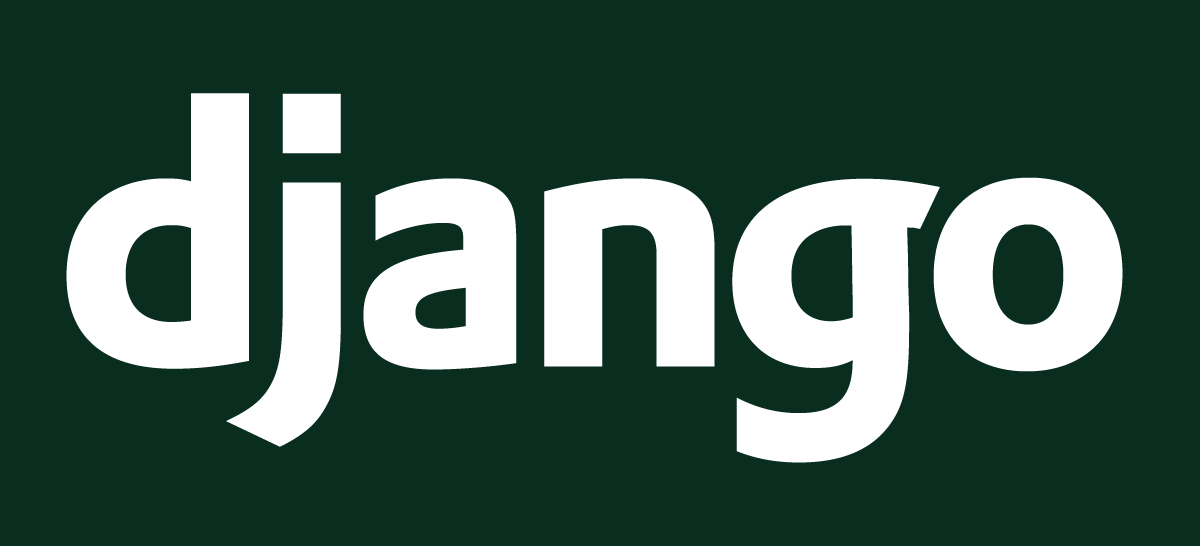
\includegraphics[width=12cm]{img/django.png}
  \captionof{figure}{Django}
\end{center}

Django là một web framework miễn phí mã nguồn mở được viết bằng Python. Django sử dụng mô hình Model-View-Control (MVC). Django được phát triển bởi Django Software Foundation(DSF) – một tổ chức phi lợi nhuận độc lập.

Mục tiêu chính của Django là đơn giản hóa việc tạo các website phức tạp có sử dụng cơ sở dữ liệu. Django tập trung vào tính năng “có thể tái sử dụng” và “có thể tự chạy” của các component, tính năng phát triển nhanh, không làm lại những gì đã làm. Một số website phổ biến được xây dựng từ Django là Pinterest, Instagram, Mozilla, và Bitbucket.

Django là một trong những framework phát triển web được yêu thích nhất cho việc phát triển các ứng dụng Python. Framework Django cho phép nguyên lý DRY (Don't Repeat Yourself) 

Không như các framework khácc, framework full-stack sử dụng miễn phí và mã nguồn mở của Python bao gồm một số lượng lớn các tính năng tích hợp thay vì cung cấp chúng dưới dạng các thư viện riêng lẻ. Django sử dụng ORM của nó để ánh xạ các đối tượng vào các bảng cơ sở dữ liệu. Điều này cho phép code hoạt động trên các cơ sở dữ liệu khác nhau cũng như giúp việc di chuyển từ cơ sở dữ liệu này sang cơ sở dữ liệu khác dễ dàng hơn. Mặc dù Django có hỗ trợ cho MySQL, PostgreSQL, SQLite và Oracle Database, nhưng nó vẫn có thể hỗ trợ các cơ sở dữ liệu khác thông qua trình điều khiển của bên thứ ba.

\textbf{Các điểm nổi bật chính:}
\begin{itemize}
    \item Học tập nhanh. Tương tự Python, Django cũng rất dễ học, không như Ruby on Rails.
    \item Tự động tạo SQL tables. Django sẽ thay bạn làm công việc này khi bạn đã xác định được cấu trúc.
    \item Tạo forms. Khi bạn đã tạo được Form class trong Django và linked đến model, form generator trong Django sẽ đảm nhận render form, xác minh và lưu trưc data.
    \item Admin Interface. Tương tự SQL table, khi bạn đã xác định được cấu trúc, Django sẽ tạo một admin interface cho phép bạn quản lý database (không khác gì PhpMyAdmin được build-in trong Django cả.)
    \item Django Shell. Python shell, ngay trong môi trường của Django project, chính là lợi thế mà Django shell mang lại. Tính năng này rất hữu hiệu khi debug (thường khó thực hiện trên PHP hơn).
\end{itemize}

\subsubsection{Framework Flask}
\begin{center}
  \captionsetup{type=figure}
  
\includegraphics[width=12cm]{img/flask.png}
  \captionof{figure}{Flask}
\end{center}

Flask là một web frameworks, nó thuộc loại micro-framework được xây dựng bằng ngôn ngữ lập trình Python. Flask cho phép bạn xây dựng các ứng dụng web từ đơn giản tới phức tạp. Nó có thể xây dựng các api nhỏ, ứng dụng web chẳng hạn như các trang web, blog, trang wiki hoặc một website dựa theo thời gian hay thậm chí là một trang web thương mại. Flask cung cấp cho bạn công cụ, các thư viện và các công nghệ hỗ trợ bạn làm những công việc trên.

Flask là một micro-framework. Điều này có nghĩa Flask là một môi trường độc lập, ít sử dụng các thư viện khác bên ngoài. Do vậy, Flask có ưu điểm là nhẹ, có rất ít lỗi do ít bị phụ thuộc cũng như dễ dàng phát hiện và xử lý các lỗi bảo mật.

\textbf{Tính năng của Framework Flask:}
\begin{itemize}
    \item Phát triển máy chủ.
    \item Phát triển trình gỡ lỗi.
    \item Hỗ trợ sẵn sàng để kiểm thử đơn vị.
    \item Jinja2 templates.
    \item RESTful request dispatch.
    \item Hỗ trợ bảo mật cookie.
    \item Full WSGI compliant.
    \item Tài liệu mở rộng.
    \item Dựa trên Unicode.
    \item Khả năng tương thích công cụ dựa trên ứng dụng Google.
    \item Nhiều tiện ích mở rộng cho các tính năng mong muốn.
    \item Tính modular và thiết kế gọn nhẹ.
    \item ORM-agnostic.
    \item Độ linh hoạt cao.
    \item Cung cấp xử lý HTTP request.
    \item API có độc đáo và mạch lạc.
    \item Dễ dàng triển khai.
\end{itemize}

\textbf{Điểm mạnh của Framework Flask:}
\begin{itemize}
  \item \textbf{Flask là một micro web framework:} Flask là một micro web framework được viết bằng Python, không yêu cầu tool hay thư viện cụ thể nào. “Micro” không có nghĩa là thiếu chức năng mà “micro” theo triết lý thiết kế là cung cấp một lõi chức năng “súc tích” nhất cho ứng dụng web nhưng người dùng có thể mở rộng bất cứ lúc nào. Flask luôn hỗ trợ các thành phần tiện ích mở rộng cho ứng dụng như tích hợp cơ sở dữ liệu, xác thực biểu mẫu, xử lý upload, các công nghệ xác thực, template, email, RESTful..., chỉ khác là khi nào bạn muốn thì bạn mới đưa vào thôi. Người dùng có thể tập trung xây dựng web application ngay từ đầu trong một khoảng thời gian rất ngắn và có thể phát triển quy mô của ứng dụng tùy theo yêu cầu.
  \item \textbf{Flask dễ cài đặt và triển khai:} Sau khi cài đặt Python, để cài đặt Flask chỉ cần bạn gõ lệnh: pip install Flask Bây giờ chúng ta thử tạo ứng dụng web với câu chào Hello World!. Thật đơn giản bạn sẽ tạo một folder với tên folder là tên ứng dụng, sau đó, tạo một tập tin .py và viết code. Flask tập trung vào sự tối giản, cho phép chúng ta xây dựng ứng dụng nhanh hơn.
  \item \textbf{Flask thật sự phù hợp cho việc xây dựng các web application có quy mô vừa và nhỏ, các API và web services:} 
  \begin{itemize}
    \item Xây dựng web application rất giống với việc viết các module Python chuẩn, cấu trúc gọn gàng và rõ ràng.
    \item Thay vì cung cấp hết tất cả mọi thứ, Flask cung cấp cho người dùng các thành phần cốt lõi thường được sử dụng nhất của khung ứng dụng web như URL routing, request and response object, template...
    \item Với Flask, việc chọn component nào cho ứng dụng là việc của chúng ta. Điều này thật tuyệt, vì mỗi web application có những đặc điểm và tính năng riêng, nó không phần phải chứa các component mà nó không dùng.
\end{itemize}
  \item \textbf{Flask giúp ta tập trung xây dựng ý tưởng, mục tiêu của riêng mình:} Flask có kiến trúc nhỏ, gọn nên bạn hoàn toàn không bị bó buộc bởi bộ khung cồng kềnh, không gặp bất cứ khó khăn nào khi cấu hình hay tổ chức ứng dụng. Không những thế, Flask còn có các ưu điểm nổi bật như: cực kỳ linh hoạt, tối giản, dễ tìm hiểu và sử dụng, định tuyến dễ dàng, rất dễ mở rộng. Vì vậy, công việc chính của ta là chỉ cần xác định ý tưởng, mục tiêu, tập trung vào việc xây dựng ứng dụng web mà thôi.
  \item \textbf{Nguồn tài liệu tham khảo về Flask rất phong phú:} Flask cung cấp rất nhiều tài liệu từ cài đặt đến thực hiện và triển khai, từ hướng dẫn nhanh đến hướng dẫn chi tiết. Ta có thể dễ dàng tìm kiếm, tham khảo, học tập về lập trình web application với Flask framework miễn phí trên Internet.
  \item \textbf{Cộng đồng Flask khá lớn:} Ta có thể dễ dàng, nhanh chóng tìm được giải pháp từ cộng đồng người sử dụng Flask mỗi khi gặp vấn đề cần giúp đỡ ví dụ như gặp lỗi, cách cài đặt thư viện, cách triển khai ứng dụng.
  \item \textbf{Mức độ phổ biến:} Có nhiều khách hàng đặt web application được xây dựng từ Flask Framework như Pinterest, LinkedIn, Twilio, Reddit, Netflix, Uber…
\end{itemize}